% 参考サイト: http://www.is.nagoya-u.ac.jp/dep-ss/phil/kukita/others/How_to_use_TeX.pdf










\documentclass[titlepage]{jsarticle}



%\usepackage[dvipdfmx, draft]{graphicx} %図の挿入(下書き)
\usepackage[dvipdfmx]{graphicx} %図の挿入
\usepackage{ascmac}  % 枠付き文章
\usepackage{amsmath} % 数式
\usepackage{comment} % 複数行コメント
% 定理
\usepackage{amsthm}
\newtheorem{thm}{定理}
\newtheorem{definition}[thm]{定義}
\newtheorem{example}[thm]{例}




% タイトル
\title{MiniSatと遺伝アルゴリズムを組み合わせた短い証明の作成}
\author{和田 翔太}
\date{\today}









% 本文
\begin{document}










\maketitle










\section{概要}










\section{導入}

\begin{figure}[t]
 	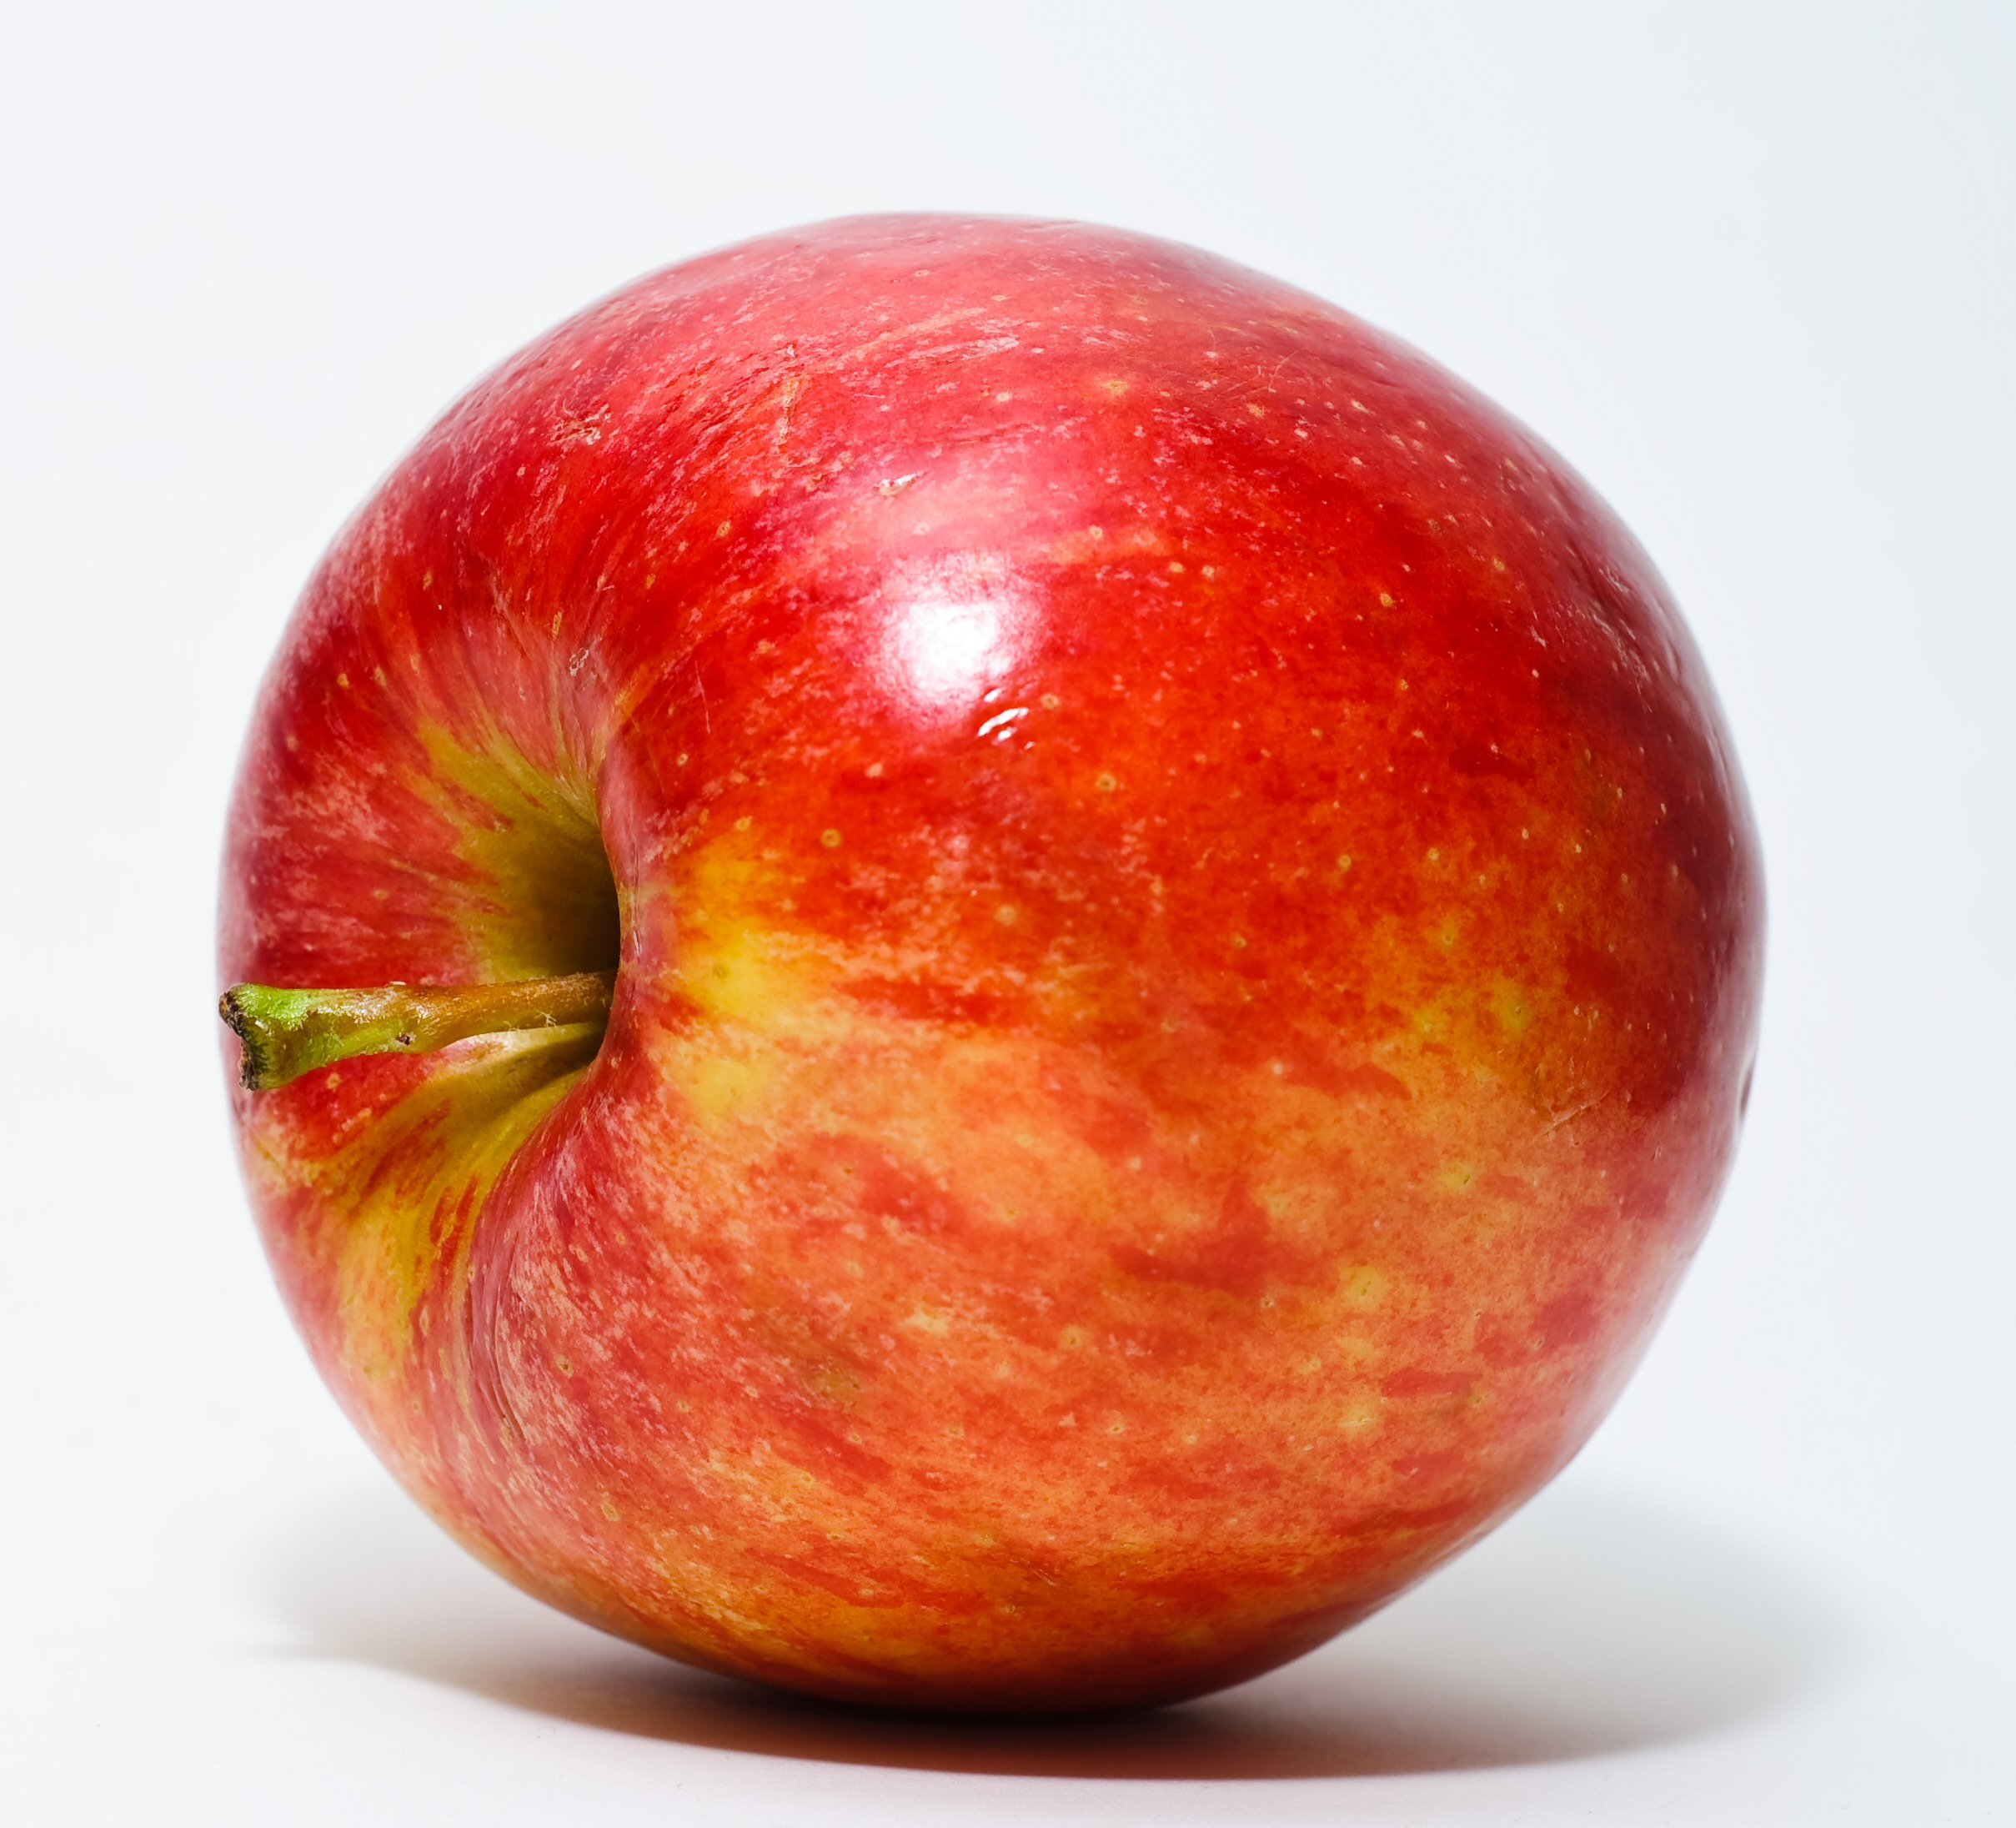
\includegraphics[width=5cm]{figures/apple.png}
	\caption{りんごの写真}
\end{figure}







\section{準備}





\subsection{SAT}



SATとは命題論理式の充足可能性を判定する問題でSatisfiability Problemの頭3文字を取ってSATと呼ばれる。
これは与えられた命題論理式を真にするような各変数への割り当てが存在するかどうか(充足可能かどうか)判定するという問題である。
命題論理式を真にするような各変数への割り当てが存在する場合は充足可能(SAT), 各変数にどのような割り当てをしても全体が真にならない場合は充足不能(UNSAT)となる。
通常SATである場合はその解(各変数への割り当て)を出力する。

\begin{definition}[命題変数]
	真を表す$\top$または偽を表す$\bot$を値にとる変数
	\[
	x_1, x_2, ...
	\]
	を命題変数と呼ぶ。
\end{definition}
命題変数それ1つでも論理式となる。
\begin{example}
	命題変数$x_1$は1変数からなる論理式となる。
\end{example}
命題論理式はこれらの命題変数を組み合わせることで表現される。

次に命題変数$x_1, x_2, ...$に対して操作を表す記号$\lor, \land, \neg$を導入する。
これらの記号は論理演算子と呼ばれ、それぞれ論理和、論理積、否定と呼ばれる。
\begin{comment}
命題変数$x_i$と$x_j$の論理和を$x_i \lor x_j$で表す。$x_i$と$x_j$がどちらも偽である場合に偽になり、それ以外の場合は真となる。
また、命題変数$x_i$と$x_j$の論理積$x_i \land x_j$で表す。$x_i$と$x_j$がどちらも真である場合に真になり、それ以外の場合は偽となる。
\[
	x_i \lor x_j = 
	\begin{cases}
		\bot & (x_i=x_j=\bot{の場合}) \\
		\top & ({それ以外の場合}) \\
	\end{cases}
	, 
	x_i \land x_j = 
	\begin{cases}
		\top & (x_i=x_j=\top{の場合}) \\
		\bot & ({それ以外の場合}) \\
	\end{cases}
\]

命題変数$x$に対してその否定を$\neg x_i$で表す。$x_i$が真である場合に$\neg x_i$は偽になり、$x_i$が偽である場合に$\neg x_i$は真となる。
\[
	\neg x_i =
	\begin{cases}
		\bot & (x_i=\top{の場合}) \\
		\top & (x_i=\bot{の場合}) \\
	\end{cases}
\]
\end{comment}

以下、$x_i$と$x_j$を命題変数とする。

\begin{definition}[論理和]
	$x_i \lor x_j$を$x_i$と$x_j$の論理和と呼ぶ。
	$x_i$と$x_j$がどちらも偽である場合に偽になり、それ以外の場合は真となる。
	\[
		x_i \lor x_j = 
		\begin{cases}
			\bot & (x_i=x_j=\bot{の場合}) \\
			\top & ({それ以外の場合}) \\
		\end{cases}
	\]
\end{definition}

\begin{definition}[論理積]
	$x_i \land x_j$を$x_i$と$x_j$の論理積と呼ぶ。
	$x_i$と$x_j$がどちらも真である場合に真になり、それ以外の場合は偽となる。
	\[
		x_i \land x_j = 
		\begin{cases}
			\top & (x_i=x_j=\top{の場合}) \\
			\bot & ({それ以外の場合}) \\
		\end{cases}
	\]
\end{definition}

\begin{definition}[否定]
	$\neg x_i$を$x_i$の否定と呼ぶ。
	$x_i$が真である場合に$\neg x_i$は偽になり、$x_i$が偽である場合に$\neg x_i$は真となる。
	\[
		\neg x_i =
		\begin{cases}
			\bot & (x_i=\top{の場合}) \\
			\top & (x_i=\bot{の場合}) \\
		\end{cases}
	\]
\end{definition}

上記の論理演算子を命題変数と組み合わせたものは論理式となる。
\begin{example}
	$\neg x_i$は1変数からなる論理式になる
\end{example}
\begin{example}
	$x_i \lor x_j, x_i \land x_j$はそれぞれ2変数からなる論理式になる。
\end{example}

論理式$X_i, X_j$に対しても命題変数と同様に論理式の論理和$X_i \lor X_j$, 論理積$X_i \land X_j$, 否定$\neg X_i$を定義することができる。

上記の3つの論理演算子とは他の演算子として排他的論理和$\oplus$, 含意$\to$, 同値$\leftrightarrow$があるが、
今回のSATの問題を表現する際に用いないので省略する。
実際には排他的論理和$\oplus$, 含意$\to$, 同値$\leftrightarrow$は全て論理和$\lor$, 論理積$\land$, 否定$\neg$を用いて表現できるため、
6つ論理演算子で表現できる論理式は全て論理和$\lor$, 論理積$\land$, 否定$\neg$を用いて表現できる。

SATの問題は通常、連言標準形(conjunctive normal form; CNF)と呼ばれる特定の形式の論理式で表現される。

\begin{definition}
	命題変数$x_i$または命題変数の否定$\neg x_i$をリテラルと呼ぶ。
\end{definition}

\begin{definition}
リテラル$l_1, l_2, ...l_n$に対してそれらを論理和$\lor$でつないだ論理式
\[
	l_1 \lor l_2 \lor ... l_n
\]
を節と呼ぶ。
\end{definition}

SATの問題(CNF式)はこの節を論理積でつないだ論理式で表現される。

\begin{definition}
	節$C_1, C_2, ...C_m$に対してそれらを論理積$\land$で繋いだ論理式
	\[
		C_1 \land C_2 \land ... \land C_m = (l_{11} \lor l_{12} \lor ... l_{1n_1}) \land (l_{21} \lor l_{22} \lor ... l_{2n_2}) \land ... \land (l_{m1} \lor l_{m2} \lor ... l_{mn_m})
	\]
	をCNF式と呼ぶ
\end{definition}

\begin{example}
	論理式$(x_1 \lor x_2) \land (\neg x_3 \lor x_4)$はCNF式である
\end{example}

\begin{example}
	論理式$(x_1 \land x_2) \lor (\neg x_3 \lor x_4)$はCNF式ではない
\end{example}

また節をリテラルの集合で表し、CNF式を節の集合で表すことがある。
先ほどの例のCNF式$(x_1 \lor x_2) \land (\neg x_3 \lor x_4)$は$\{\{x_1, x_2\}, \{\neg x_3, x_4\}\}$といった集合で表現される。

最後に充足可能、充足不能について定義する。

まず割当を定義する。
\begin{definition}[割当]
命題変数についてその割当(未割当も含める)を写像
	\[
		\nu: X \to \{\top, \bot, u\} (X{は命題変数の集合とし、}u{は未割当であることを表す})
	\]
で定義する。
\end{definition}

この写像$\nu$をリテラル$l$, 節$C=\{l_1, l_2, ..., l_n\}$, CNF式$F=\{C_1, C_2, ..., C_m\}$についても割当ができるように以下のように拡張する。
\begin{definition}
	\begin{align*}
		\nu(l) & = 
		\begin{cases}
			\nu(x)     & (l= x{の場合}) \\
			\neg\nu(x) & (l=\neg x{の場合}) \\
		\end{cases}
		({ただし}\neg u = u{とする}) \\
		\nu(C) & = \nu(l_1) \lor  \nu(l_2) \lor  ... \lor  \nu(l_n) \\
		\nu(F) & = \nu(C_1) \land \nu(C_2) \land ... \land \nu(C_m)
	\end{align*}
\end{definition}

この割当を用いて充足可能と充足不能を定義する

\begin{definition}[充足可能]
	CNF式$F$に対して充足可能(SAT)とはある割当$\nu$が存在して
	\[
		\nu(F) = \top
	\]
	となることをいう。
\end{definition}

\begin{definition}
	CNF式$F$に対して充足不能(UNSAT)とは任意の割当$\nu$に対して
	\[
		\nu(F) = \bot
	\]
となることをいう。
\end{definition}



\begin{example}
	$ (x_1 \lor x_2) \land (x_1 \lor \neg x_2) \land (\neg x_1 \lor \neg x_2) $はSATである。
	これを充足する割当$\nu$の例としては$x_1=\top$, $x_2=\bot$が挙げられる。
\end{example}

\begin{example}
	$(x_1 \lor x_2) \land (\neg x_1 \lor x_2) \land (x_1 \lor \neg x_2) \land (\neg x_1 \lor \neg x_2)$はUNSATである。
	変数$x_1,x_2$に真偽値を割当てる方法は合計で$4$つあるが、そのいずれもこの論理式を充足しないことが確認できる。
\end{example}




\subsection{SAT solver}
充足可能性問題を解くソルバーのことをSAT solverと呼ぶ。
充足可能性問題はNP完全に属し、解くのに時間がかかる。% 時間がかかることを説明したい
一番愚直な解き方として、各変数に$\top$と$\bot$を代入して全体が真になるかどうかを判断する方法がある。
しかしこの場合最悪$2^n$回確認をしなければならない。
そのため、速く解くために様々な手法が用いられる。





\subsubsection{単位伝搬}
後述するDPLLアルゴリズムの説明の際に用いられる単位伝搬について説明する。
まずは単位節について説明をする。
\begin{definition}

\end{definition}





\subsubsection{DPLLアルゴリズム}
DPLL(Davis-Putnam-Logemann-Loveland)アルゴリズムとは単位伝搬(Unit propagation)を用いたアルゴリズムのことである。
CNF式の命題論理式は各節が論理積で繋がった形をしているため、全体が真となるためにはその各節が真とならなければならない。
もし仮にある節において、1つのリテラルのみが未定義でその他のリテラルが偽になる場合($x \land \bot \land \bot ...$)、その節が真になるためには未定義のリテラルが真にならなければならない。
このようにして未定義のリテラルが真になるように割り当てを行うことを単位伝搬という(またそのような節を単位節と呼ぶ)。
DPLLアルゴリズムは以下のような流れで問題を解いていく
\begin{enumerate}
	\item 単位節がある場合、それを充足するように変数に割り当てを行う(単位伝搬)
	\item 単位節がない場合、適当な変数を選択し真または偽を割り当てていく
	\begin{itemize}
		\item 割り当てによって単位節ができた場合、単位伝搬を行う
		\item 矛盾が発生した場合、最後に選択していた変数の真偽値を反転(すでに反転していた場合はその1つ前の変数を反転)させる
	\end{itemize}
	\item 全体が真になった場合はSAT(とその割り当て)を、すべての割り当てにおいて全体が偽になった場合はUNSATを返す
\end{enumerate}



\subsubsection{変数選択における重み}
DPLLアルゴリズムにおいて変数選択をする際に未割当の変数が複数ある場合、どの変数を選択すべきかという問題がある。
一番シンプルな方法としてランダムに選ぶ方法もあるが、実際にはどのようにして変数を選択するかが決まっている。
多くのソルバーにおいてはあるルールに従って各変数に重み(スコア)をつけることで変数選択をする時に重みが一番大きい変数を選択するようになっている。
後述するソルバーの1つであるminisatにおいては、矛盾が発生した際にその矛盾を引き起こすのに関わった変数(その時に作った学習節に含まれる変数)のスコアが上がるように計算することで、
直近の矛盾に関わった変数ほどスコアが高くなっている。
変数選択の際には一番重みが大きい変数を選択している。



\subsubsection{矛盾からの節学習(CDCL solver)}
DPLLアルゴリズムに基づいた高速SAT solverの大きな特徴であり、
これを用いたsolverはしばしばCDCL(conflict-driven clause learning) solverと呼ばれる。
節学習の流れとして、まず、DPLLアルゴリズムにおいて矛盾が起きた際にどの変数への割り当てが矛盾を引き起こしたのかなどの原因を調べる。
そして今後変数割当や単位伝搬を進めていく中でさきほどの矛盾を引き起こした変数らへの割当を防ぐために
新しい節を学習節として新しく節を加える。
これを続けていくことでDPLLアルゴリズム単体で解の探索をするよりも高速に探索をすることができる。
なお、探索が長時間に及ぶ場合には学習節の数が膨大になる可能性があり、メモリ確保のために一定量の学習節を定期的に削除している。



\begin{comment}
\subsubsection{監視リテラル}
SAT solverの実行時間の70\%から90\%は単位伝播の処理で占められているため、効率良く単位節を検出することができればより高速に解を探索することができる。
素朴な方法として各変数$x_i$に対して$x_i$を含む節のリストを用意しておき、
$x_i$に値が割り当てられた時にそのリストを走査することで状態の変化した節を確認する方法がある。
しかしこの方法だとすでに充足されている節の確認を行う必要があり無駄が多くなってしまう。
監視リテラルを用いた方法は節の中の未割当な変数2つを監視する方法である。
節が単位節になる直前の状態は節中のリテラルのうち2つのみが未割当で残りのリテラルに偽が割り当てられている状態となっている。
どちらかのリテラルに偽が割り当てられた時に節は単位節となるため、
節中の全てのリテラルを監視する必要はなく未割当のリテラル2つのみを監視するだけで効率良く単位節を検出することができる。
\end{comment}





\subsection{DRAT}
DRAT(Deletion Resolution Asymmetric Tautology)とは証明の表記法の1つであり、
DRUP(Deletion Reverse Unit Propagation)と呼ばれる証明の表記法を一般化したものである。
数学の問題を証明する際にいくつかの補題を組み合わせて証明をするように、
DRATの証明も主にいくつか補題を表す節を並べることで作成される。
DRATの証明の各行は、補題を表す節かそれまでにある特定の節を削除する意味を持つ削除節からなり、
最後の行は矛盾を表す長さ0の節(リテラルを1つも持たない節)となっている。
ここで証明の検証方法を説明するためにいくつか変数を取り入れる。
CNF形式の問題を$F$、CNF形式の証明を$P$として、証明が持つ節の数(証明の行数)を$|P|$とする。
$i \in \{0,1,...,|P|\}$に対して$F_{P}^{i}$を次のように定義する。
ただし、$L_i$を証明$P$における$i$行目の節とする。
\[
	F_{P}^{i} = 
	\begin{cases}
		F                           & (i=0{の場合}) \\
		F_{P}^{i-1} \setminus \{L_i\} & (L_i{が削除節の場合}) \\
		F_{P}^{i-1} \cup      \{L_i\} & ({それ以外}) 
	\end{cases}
\]
証明を検証する際には、証明の各行の節をRUPチェックとRATチェック両方で検証を行いその節を導くことができるかを検証する。
\begin{description}
	\item[RUPチェック] $F_{P}^{i-1}$に関して$L_i$を単位伝搬のみで導出することができる
		($F_{P}^{i-1} \cup \{\overline L_i\}$について単位伝搬のみで矛盾を導くことができる)
	\item[RATチェック] $F_{P}^{i-1}$に関して$L_i$が$l_i$について以下の性質を持っているか \\
		\begin{itemize}
			\item 任意の$C \in F_{P}^{i-1}$について$\overline l_i$が$C$に含まれる場合、
				$F_{P}^{i-1}$に関して$(C \setminus {\overline l_i}) \cup L_i$を単位伝搬のみで導出することができる。
		\end{itemize}
\end{description}
実際に検証するツールとしてdrat-trimが存在する。
このツールのもう1つの特徴として元の証明を短くすることができる。
検証を行う際にもとの証明の中で使用されなかった節を削除する方法で元の証明よりも短い証明を出力している。



\subsubsection{学習節とDRAT}
CDCLソルバーが作成する学習節はこのDRATの証明になっている。
先ほど述べたように、学習節は以降の探索の際に矛盾を引き起こした割当になることを防ぐ役割を持っている。
例えば学習節$C$が$l_1 \lor l_2 \lor ... \lor l_n$を形をしているとする。
この学習節が作られた際には$l_1=\bot, l_2=\bot, ... , l_n=\bot$という割当によって矛盾が引き起こされていたことがわかる
($\overline C = \overline l_1 \land \overline l_2 \land ... \land \overline l_n$)。
つまり$\overline C$を仮定した時に単位伝搬のみで矛盾を導くことができるため、RUPチェックによってこの学習節を導くことができる。
したがって、CDCLソルバーが問題を解く際に作成されていく学習節を並べていくと問題がUNSATである時のDRATの証明になっている。
この作り方において、証明の中に削除節は存在しない(後述する今回の実験で使うソルバーにおいては削除節が作成される)。



\subsubsection{証明の長さ}
実験の目標とする短い証明を作ることについて、ここでは証明の長さを証明の節の中で補題を表す節の数で表す。
削除を表す節はそれ自体が存在しなくても証明として成り立つため、削除を表す節については考慮しない。





\subsection{minisat}



SATソルバーの1つであり、今回証明を作成するのに使用しているソルバーである。

特長の1つとして詳細を理解しやすいという点がある。
既存の最先端のソルバーを改良することは、仮に問題領域やSATソルバーに関する技術を深く理解していても10000行を超えるプログラムを理解しなければならず、極めて時間のかかる作業になってしまう。
同様にゼロからソルバーを構築しようとしても多くの時間を費やす必要がある。
このように時間がかかってしまう理由としては、現代のソルバーで用いられている技術は十分に文書化されている一方で、
実装に必要な詳細が十分に提示されていないことが挙げられる。

これに対してminisatは
\begin{itemize}
	\item プログラム全体のコード行が6000行と比較的少ない
	\item 矛盾からの節学習、監視リテラル、変数への重み付けといった既存のソルバーに多く採用されている技術が使用されている
	\item 実装の詳細について説明した論文が存在する
	\item オープンソースである
\end{itemize}
ため、改造がしやすかったり独自のソルバーをゼロから構築しやすくなっている。

今回は変数選択へ介入を行うため、ソルバーの改造が必要であるという理由から、minisatを使用した。





\subsection{遺伝アルゴリズム}



遺伝アルゴリズム(G.A.: genetic algorithm)とは、John Hollandによって発明された、最適化アルゴリズムのことである。
このアルゴリズムは自然進化に見られる過程のいくつかを模倣して構築されている。
この進化は染色体と呼ばれる生物の構造を符号化するための有機的な装置上で生じており、
1個体の生物は染色体を翻訳する過程により作られる。
染色体のコード化と翻訳の過程の特徴として、
\begin{itemize}
	\item {進化は生命体そのものにではなく、それを符号化した染色体に対して操作を行う過程からなる}
	\item {自然淘汰は、染色体とそれをデコードした結果できた構造体の環境への適応度を結びつける。
	この過程により、より適応した染色体はより頻繁に再生に用いられる。}
	\item{再生と呼ばれる今ある染色体から新しい染色体を生成する操作の過程で、進化が起きると考えられる。
	突然変異と呼ばれる操作によって親のものとは異なった染色体が生成され、
	組み替えの過程を通して両者の染色体の構成物質が組み合わされてどちらの親の特徴を持つ全く異なった染色体が作られる。}
\end{itemize}
といった特徴がある。



\subsubsection{遺伝アルゴリズムの概観}

まず最初に遺伝アルゴリズムを今解きたい問題と結びつけるためにどのような機構が必要か考える。
この機構は主に2つあり、問題の解を染色体上に変換するコード化の部分と、染色体がどれだけその問題において優秀なのかの度合いを返す評価関数の部分である。

どのようにコード化するかについては様々な手法があり、1つの例としてはビット列で表現する方法などがある。
おそらく全ての問題に対して最良であるような手法は存在せず、問題によって適切な表現を使用することが求められる。

遺伝アルゴリズムと問題を結びつける評価関数は染色体を入力とし、問題に関する評価の度合いを表す数または数のリストを返す。
評価関数は自然進化における環境と同様の役割を果たしており、染色体と評価関数との相互作用によって遺伝アルゴリズムが再生を行う際に用いる適応の度合いを与えることができる。

また遺伝アルゴリズムを構築する前に考える必要がある機構として、新しい子を作成する際にどのような交叉とどのような突然変異を用いるかについて考える必要がある。
交叉は2つの親から2つの子を生成する操作であり、遺伝子を一部交換し親の遺伝情報を掛け合わせてより良い個体を生成する。
この結果親に似た個体を生成することができる。
突然変異は遺伝子の1部分をランダムに変動させる操作であり、これによって探索空間内の探索範囲を限定してしまうことを回避したり、局所解から脱出する効果がある。

\hfill \break
\begin{itembox}[c]{遺伝アルゴリズムの概観}
	\begin{enumerate}
		\item 染色体の集団を初期化する。
		\item 集団の各染色体を評価する。
		\item 現在の染色体を組み合わせて新しい染色体を生成する。この時交叉と突然変異を親の染色体に適用することで新しい染色体を生成する。
		\item 新しい染色体の入る場所をあけるために集団の一部を削除する。
		\item 新しい染色体を評価し、集団に挿入する。
		\item 決められた時間が経過したら、停止する。そうでない場合は3に戻る。
	\end{enumerate}
\end{itembox}
\hfill \break


これらの初期の構成をどのようにするかが決まると遺伝アルゴリズムを用いて解の集団の擬似進化を実現することができる。
上記の図は遺伝アルゴリズムの概観について説明したものである。
もしこの擬似進化の過程がすべてうまくいったのであれば、普通の染色体からなる初期集団は親がより良い子によって置き換えられていくにしたがって集団全体がより良い染色体たちになっていくことが期待される。
そして、最後に生成された集団での最良の個体はその問題に対する高度に進化した解になることが期待される。










\section{実装}





実験を行うにあたっていくつかの実装を行なった。





\subsection{証明を作る}



今回の研究においては証明が必要不可欠であり、使用したいソルバーが証明を作成しない場合、そのままの状態では実験に使用することができない。
minisatには証明を出力してファイルに保存する機能が存在しなかったので既存のminisatを改造することで証明を出力できるようにした。
上述したようにこの証明を出力させる方法としてCDCLソルバーが作成する学習節を順にファイルに追加していくことで証明を作ることができるのだが、
minisatにはこの学習節以外にも新しく節を作成している部分が存在するためこのままでは証明として成立してない。
minisatは問題の解を探索する前に、より効率的に探索をするために前処理という操作を行なっている。
この前処理の段階でminisatは問題にあるいくつかの節を組み合わせたりしながら新しい節を作成している。
そのため、この新しく作成した節も証明の中の節として出力する必要がある。
この2種類の方法で作成される節を出力していくことで証明ファイルを作成できるように実装を行なった。

また、minsatが不要な節を削除する際には削除節を追加して、のちのdrat-trimの実行時間を短縮している。
minisatが学習節を削除する部分は主に2つで、1つ学習節が膨大になった場合に学習節を削除する部分と前処理の段階ですでに真になっている節を削除する部分である。





\subsection{変数選択への介入}



続いて、minisatの変数選択に介入を行なった。
準備の部分で述べたように、minisatは各変数にスコアを割り当てており、変数選択を行う際にこのスコアが1番高い変数を選ぶ仕組みになっている。
この変数のスコアを変更するように介入を行なった。
具体的には何回目かの変数選択時にスコアを変更するかのタイミングを指定して、探索の中で実際にその変数選択の回数が指定した回数になった時に各変数のスコアをランダムに書き換えてから変数選択を行う。
書き換えるスコアは0以上1以下の値をランダムに選んだ。
この書き換えによって後の選択する変数などが変化する。

また、後述する遺伝アルゴリズムと組み合わせる際には一度行なった介入を再度行わなければならない可能性がある。
つまり一度書き換えた各変数のスコアを再現しなければならない。
変数のスコアを全て保存しておいて、同様の介入を再現する際に全てのスコアを読み取って書き換える方法があるが、
変数が多い場合にはサイズが莫大な大きさになってしまう。
今回はスコアを全て保存するのではなくその値を割当てる前にシード値を保存しておき、同様の介入を再現する場合には書き換える前にシード値を保存したシード値に変更してから書き換えを行なうような形で同様の介入を再現した。

したがって、minisatの変数選択に介入する際には
\begin{itemize}
	\item 介入のタイミング(何回目の変数選択で介入を行うか)
	\item ランダムで書き換えることを指定する値、または一度行なった介入を再現するためのシード値
\end{itemize}
の2つを指定することで変数選択に介入を行えるようにminisatを改造した。
複数回介入を行う際にはこの2つの値を並べることで複数回の介入を行うことができる。





\subsection{遺伝アルゴリズム}



ここからは準備で述べた遺伝アルゴリズムを今回の実験においてどのように実装を行うかについて説明する。

まず最初に考えるべき部分として染色体をどのように表現するかという部分と評価関数をどのように定義するかという部分がある。
今回はタイミングと書き換え方法を表す値を1つの組にしたものを1つの介入として、この介入を並べた介入列を染色体とした。
この時介入のタイミングの上限は、介入なしで解かせた時の変数選択数とした。
また、評価関数については染色体(介入列)を受け取ってその介入のもとでminisatを実行してからdrat-trimを実行した後にできる証明の長さを返す関数とした。

続いて新しい子を作成する際に用いる交叉と突然変異のオペレータについて考える。
交叉については、2つの親に対してある1点を指定してそれ以降を交換する1点交叉を使用した。
具体的にはタイミングをランダムに指定して、そのタイミング以降の介入列を交換するようにした。
突然変異については、新しい介入を1つ追加する突然変異と今ある介入の中から1つ削除する突然変異の2つを採用した。

その他細かい部分として新しい子を生成する際の親の選択方法としては、各染色体の評価値の逆数を重みとしてランダムに選択している。
つまり短い証明を作成するような染色体ほど親として選ばれやすいようになっている。
また新しい世代の作り方としては既存の集団の一部分を削除して空いた部分に新しく生成した子を入れて作るのではなく、
既存の集団を全て削除して新しく生成した子で全て入れ替えるようにしている。

実装における細かい部分としては、遺伝アルゴリズムの実行後の結果ファイルの作成時に調整を行なった。
遺伝アルゴリズム実行後のデータとして、各世代各染色体の証明の長さをリストにしたデータと各世代各染色体の介入列などの全情報も含めたデータを作成しているが、
後者のデータに関しては染色体の介入列の長さが大きくなった際に全体のデータ量が大きくなってしまう問題がある。
この問題を解消するために各世代各染色体の情報をデータに収めるのではなく、その染色体を作るためにどのような交叉をしたかやどのような突然変異をしたかなどの復元のための情報をデータに収めるようにした。
復元の際に時間がかかるものの、全染色体の介入列の情報など全ての情報を復元によって手に入れることができる。
加えて交叉や突然変異の方法が大きく変わらない(復元のための情報が大きくならない)限り、染色体の介入数がどれだけ大きくなっても一定サイズのデータで出力することができる。




\section{問い}










\section{実験}










\section{結果}










\section{考察}










\section{まとめ}










\end{document}